%!TEX options = -shell-escape

\documentclass[glossy]{beamer}

% Fonts
\usepackage[utf8]{inputenc}
\usepackage{lmodern}
\usepackage[T1]{fontenc}
\usepackage{soul}

% Beamer
\useoutertheme{wuerzburg}
\useinnertheme[realshadow,corners=2pt,padding=2pt]{chamfered}
\usecolortheme{shark}

\setbeamertemplate{navigation symbols}{}

% Tikz
\usepackage{tikz}
\usetikzlibrary{tikzmark, arrows, decorations, decorations.pathreplacing, positioning}
\tikzset{every picture/.style={font issue=\scriptsize},
         font issue/.style={execute at begin picture={#1\selectfont}}
}

\tikzstyle{callout}=[remember picture, ->, >=stealth, overlay, red, ultra thick, align=center, anchor=west]

\tikzstyle{codebox}=[rectangle, draw=black, very thick, minimum size=7mm]

% Minted
\usepackage{minted}
\newminted{cpp}{autogobble, fontsize=\large, escapeinside=@@}
\newmintedfile{cpp}{autogobble, fontsize=\tiny, escapeinside=@@}
\newmintedfile{cmake}{autogobble, fontsize=\tiny}
\newmintinline{cpp}{escapeinside=@@}
\newmintinline{java}{}
\newmintinline{js}{}
\usemintedstyle{vs}

% GraphicX
\usepackage{graphicx}
\graphicspath{{img/}}

% Macros
\newcommand{\cppref}[2]{\href{http://en.cppreference.com/w/cpp/#1}{\underline{#2}}}
\newcommand{\refer}[1]{([shift={(.25em,.25em)}]pic cs:#1)}
\newcommand{\filename}[1]{\texttt{\textbf{\emph{#1}}}}

\usepackage[svgpath=img/]{svg}
\usepackage[linewidth=1pt]{mdframed}
\usepackage{color}

% Meta
\title{C++ Boot Camp 2/2}
\author{Jesse Talavera-Greenberg}
\date{}

\begin{document}

\begin{frame}[fragile=singleslide]
  \frametitle{C++ Boot Camp 2/2}
  \begin{figure}
    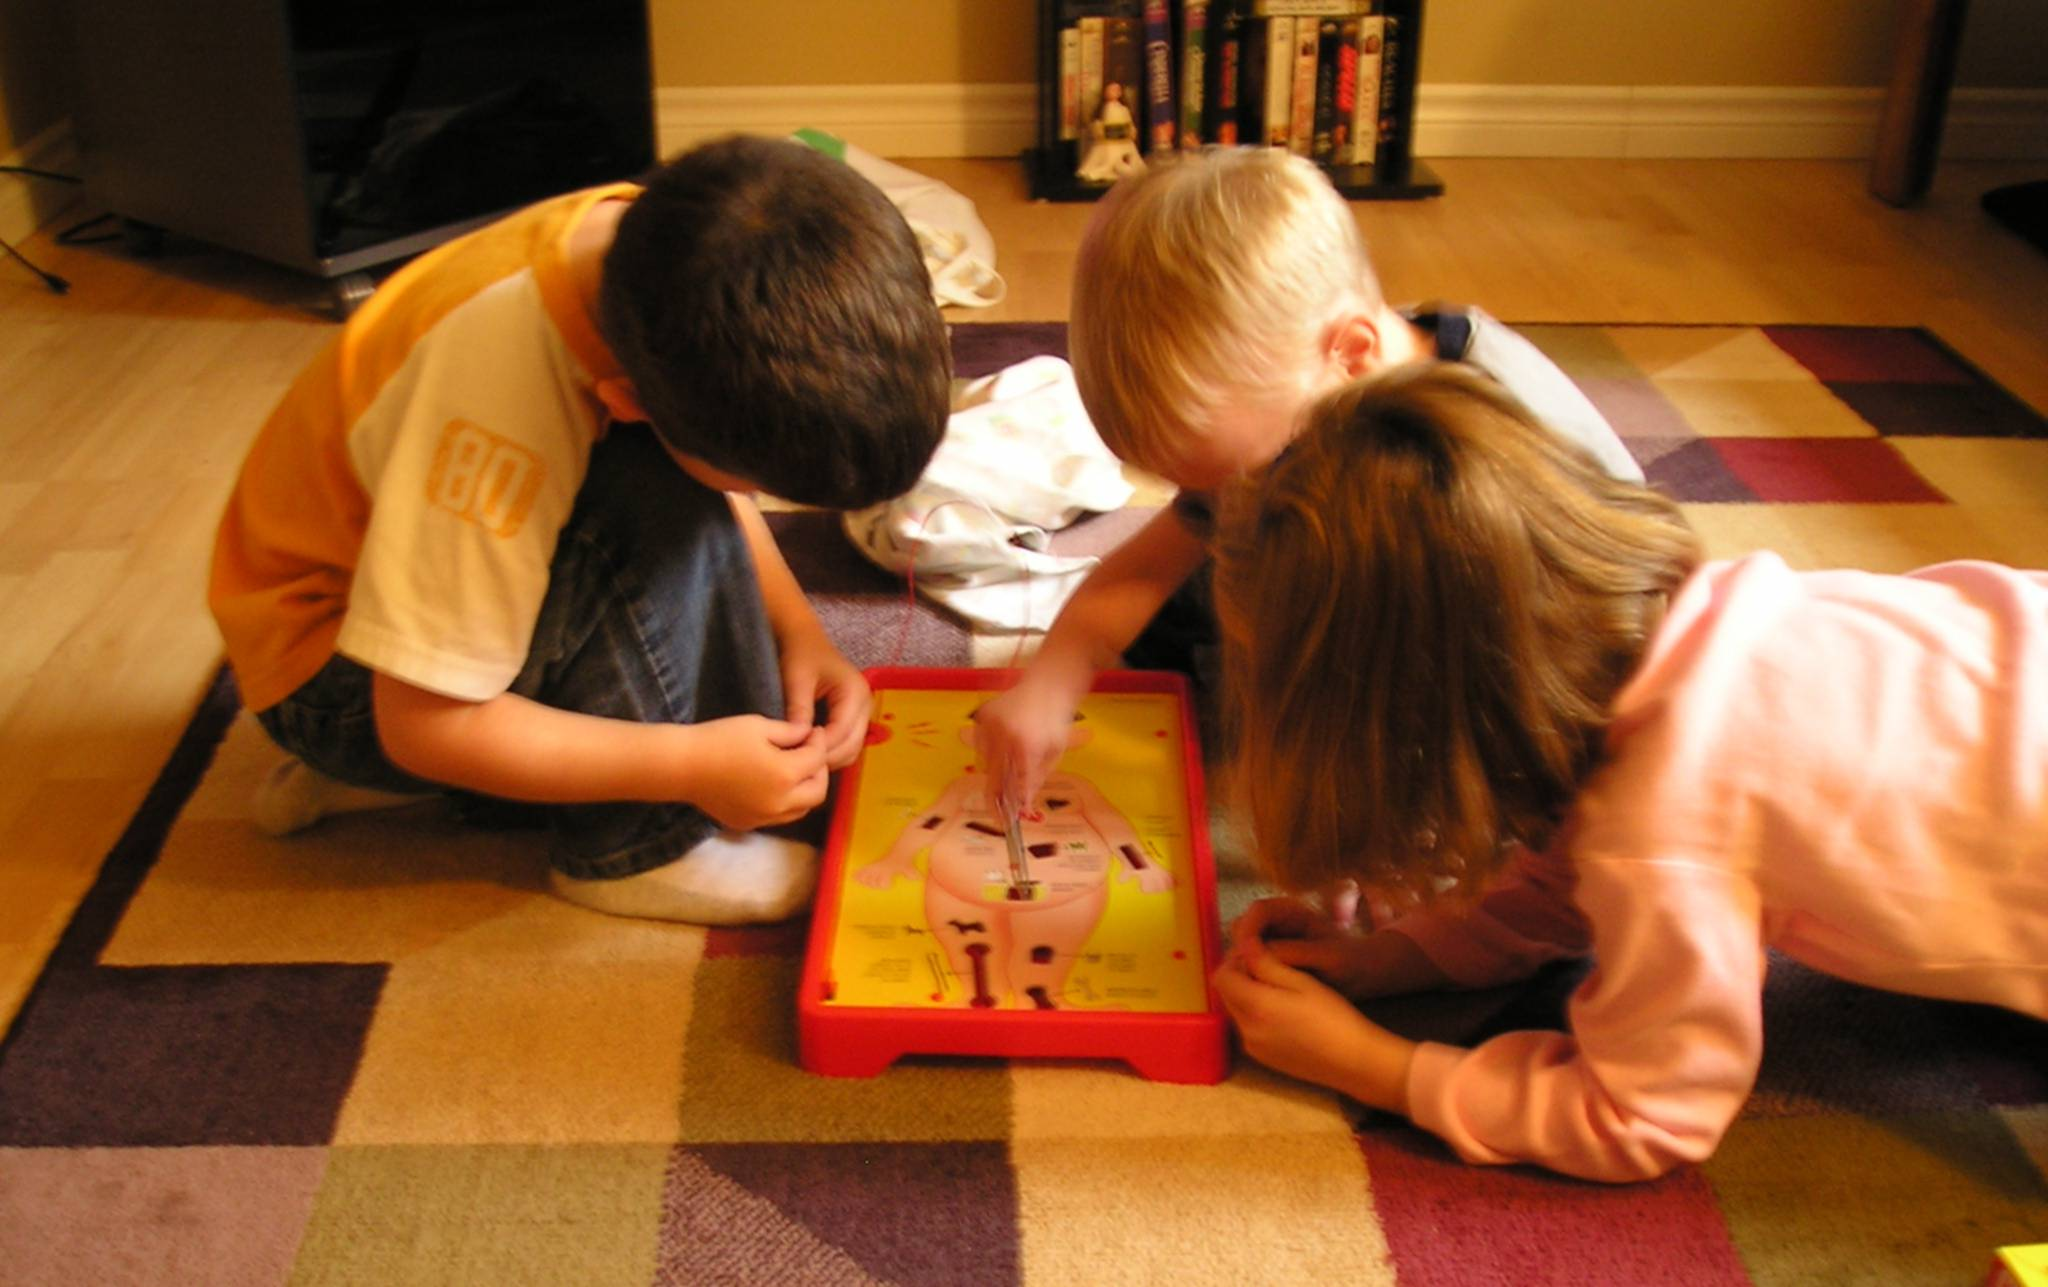
\includegraphics[width=.9\columnwidth]{operation}
    \centering
  \end{figure}
  \begin{tikzpicture}[callout, line width=2mm]
    \draw (4, 3.5) node (team) [anchor=east] {\LARGE \textbf{Your Team}} -> (4.5, 4.8);
    \draw (team.east) -> (6.5, 5);
    \draw (team.east) -> (7, 4);
    \draw (7.75, 1.5) node (team) [anchor=north west] {\LARGE \textbf{C++}} -> (6.45, 2.85);
  \end{tikzpicture}
\end{frame}

%%%%%%%%%%%%%%%%%%%%%%%%%%%%%%%%%%%%%%%%%%%%%%%%%%%%%%%%%%%%%%%%%%%%%%%%%%%%%%%

\begin{frame}[fragile=singleslide]
  \frametitle{Same Disclaimers Apply}
  \begin{itemize}
    \item I am not the grader for this course.
    \item This boot camp is entirely voluntary.
    \item Any opinions expressed are my own.
    \item I don't know much about DirectX.
    \item Correctness is likely, but \textbf{not guaranteed}.
  \end{itemize}
\end{frame}

%%%%%%%%%%%%%%%%%%%%%%%%%%%%%%%%%%%%%%%%%%%%%%%%%%%%%%%%%%%%%%%%%%%%%%%%%%%%%%%

\begin{frame}[fragile=singleslide]
  \frametitle{This Week}
  \begin{itemize}
    \item \textbf{Last week:} The language
    \item \textbf{This week:} The tools
    \item Compiling and linking, specifically Box2D
    \begin{itemize}
      \item You will be using it for your course project
    \end{itemize}
    \item Splitting classes into headers and source files
    \begin{itemize}
      \item What that means and why you must do it
    \end{itemize}
    \item Overview of popular C++ libraries and tools
    \item Tips about the course
  \end{itemize}
\end{frame}

%%%%%%%%%%%%%%%%%%%%%%%%%%%%%%%%%%%%%%%%%%%%%%%%%%%%%%%%%%%%%%%%%%%%%%%%%%%%%%%

\begin{frame}[fragile=singleslide]
  \frametitle{Declarations and Definitions}
  \begin{columns}[t]
    \begin{column}{6cm}
      \textbf{Declarations:}
      \begin{itemize}
        \item "This thing exists!"
        \begin{itemize}
          \item Usually a class or function
        \end{itemize}
        \item Defines interface only, not definition
        \begin{itemize}
          \item For classes, not even
        \end{itemize}
        \item Definition usually in another file
      \end{itemize}
    \end{column}

    \begin{column}{6cm}
      \textbf{Definitions:}
      \begin{itemize}
        \item The actual code
        \item Must match declaration
      \end{itemize}
    \end{column}
  \end{columns}

  \begin{columns}[t]
    \begin{column}{6cm}
      \cppfile{src/decl.hpp}
    \end{column}

    \begin{column}{6cm}
      \cppfile{src/defn.hpp}
    \end{column}
  \end{columns}

  
\begin{tikzpicture}[callout]
    \draw (3cm, 14em) node {Class \emph{declaration}} -> \refer{decl_forward};
    \draw (8cm, 15em) node [anchor=south] {Class \emph{definition}} -> \refer{decl_class};
    \draw (11cm, 16em) node [anchor=south] {Method\\\emph{declaration}} -> \refer{decl_decl};
    \draw (4cm, 8em) node [anchor=east] {Method declaration\\\emph{and} definition} -> \refer{decl_defn};
    \draw (11.5cm, 10em) node [anchor=south] {Method\\\emph{definition}} -> \refer{decl_decl_defn};
    \draw (1cm, 3em) node [anchor=north] {Function\\\emph{declaration}} -> \refer{decl_func};
    \draw (4cm, 3em) node [anchor=east] {Function\\\emph{definition}} -> \refer{decl_func_defn};
  \end{tikzpicture}

\end{frame}

%%%%%%%%%%%%%%%%%%%%%%%%%%%%%%%%%%%%%%%%%%%%%%%%%%%%%%%%%%%%%%%%%%%%%%%%%%%%%%%

\begin{frame}[fragile=singleslide]
  \frametitle{Compiling}

  \begin{figure}
    \centering
    \includesvg[width=\paperwidth, pretex=\scriptsize]{compiling}
  \end{figure}

\end{frame}

%%%%%%%%%%%%%%%%%%%%%%%%%%%%%%%%%%%%%%%%%%%%%%%%%%%%%%%%%%%%%%%%%%%%%%%%%%%%%%%

\begin{frame}[fragile=singleslide]
  \frametitle{Symbol Tables}

  \begin{figure}
    \centering
    \resizebox{3cm}{!}{\input{img/symbols}}
  \end{figure}

  \begin{tikzpicture}[callout]
    \draw (3,2.5) node [anchor=east] {Have: \texttt{stooge::slap}} -> (4.75,2.5);
    \draw (4,4) node [anchor=east] {Have: \texttt{std::vector<float>}} -> (6,4);
    \draw (4,1) node [anchor=east] {Seeking: \texttt{std::sin}} -> (6.5,2);
    \draw (9,2.5) node {Seeking: \texttt{stooge::poke}} -> (7,2.5);
  \end{tikzpicture}

  \begin{itemize}
    \item Multiple gaps seeking one symbol: Perfectly normal
    \item Multiple tabs declaring one symbol: \textbf{multiple definition of symbol}
    \item Gap without a tab filling it: \textbf{unresolved external symbol}
    \item Tab not assigned to a gap: Unused symbol (can be stripped)
  \end{itemize}
\end{frame}

%%%%%%%%%%%%%%%%%%%%%%%%%%%%%%%%%%%%%%%%%%%%%%%%%%%%%%%%%%%%%%%%%%%%%%%%%%%%%%%

\begin{frame}[fragile=singleslide]
  \frametitle{Linking}

  \begin{figure}
    \centering
    \resizebox{\columnwidth}{!}{\input{img/linking}}
  \end{figure}
\end{frame}

%%%%%%%%%%%%%%%%%%%%%%%%%%%%%%%%%%%%%%%%%%%%%%%%%%%%%%%%%%%%%%%%%%%%%%%%%%%%%%%

\begin{frame}[fragile=singleslide]
  \frametitle{Static and Dynamic Libraries}
  \begin{columns}[t]
    \begin{column}{6cm}
      \textbf{Static:}
      \begin{itemize}
        \item \texttt{.a} or \texttt{.lib} extension (varies by compiler)
        \item Resolved at link-time
        \item Stored in executable
        \item Must rebuild to update library
        \item Unused code can be removed
      \end{itemize}
    \end{column}

    \begin{column}{6cm}
      \textbf{Dynamic:}
      \begin{itemize}
        \item \texttt{.dylib}, \texttt{.dll}, or \texttt{.so} extension (varies by OS)
        \item Resolved at run-time
        \item Stored in program directory or system folders
        \item Can freely swap out versions
        \item Multiple programs can share code at once
      \end{itemize}
    \end{column}
  \end{columns}
\end{frame}

%%%%%%%%%%%%%%%%%%%%%%%%%%%%%%%%%%%%%%%%%%%%%%%%%%%%%%%%%%%%%%%%%%%%%%%%%%%%%%%

\begin{frame}[fragile=singleslide]
  \frametitle{My First \href{http://box2d.org/}{\underline{Box2D}}}
     
  \begin{itemize}
    \item You installed \href{https://www.visualstudio.com/downloads/download-visual-studio-vs}{\underline{Visual Studio Community 2015}}, right?
    \item \href{https://github.com/JesseTG/Box2D/archive/master.zip}{\underline{Download}} and extract somewhere
    \item Open \texttt{Build/vs2013/Box2D.sln}
    \begin{itemize}
      \item Projects contain related code
      \item Solutions contain related projects
    \end{itemize}
    \item \emph{Right-click \textbf{Box2D}} $\rightarrow$ \emph{Build}
    \item You just built a static library!
  \end{itemize}

  \begin{columns}
    \begin{column}{6cm}
      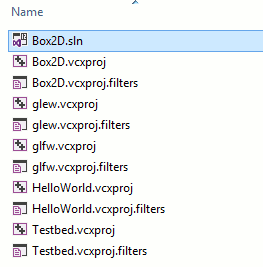
\includegraphics[width=0.9\columnwidth]{windows-03}
    \end{column}

    \begin{column}{6cm}
      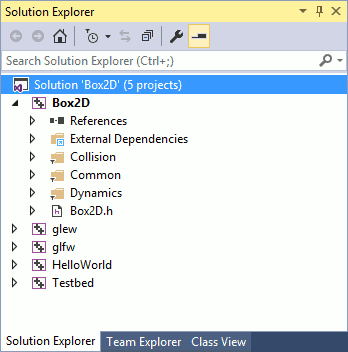
\includegraphics[width=0.9\columnwidth]{windows-04}
    \end{column}
  \end{columns}

  \begin{tikzpicture}[callout]
    \draw (1.7, 4.65) -> (6.25, 4.25);
    \draw (2.1, 4.25) -> (6.5, 3.9);
    \draw (5, 2.5) node [anchor=east] {\texttt{\#include} this\\to use Box2D} -> (6.8, 2.25);
  \end{tikzpicture}
\end{frame}

%%%%%%%%%%%%%%%%%%%%%%%%%%%%%%%%%%%%%%%%%%%%%%%%%%%%%%%%%%%%%%%%%%%%%%%%%%%%%%%

\begin{frame}[fragile=singleslide]
  \frametitle{Compiling Box2D (cont'd)}

  \begin{itemize}
    \item Do the same with Testbed
    \begin{itemize}
      \item Its dependencies are compiled for you
      \item \emph{\textbf{Solution 'Box2D'}} $\rightarrow$ \emph{Properties} $\rightarrow$ \emph{Project Dependencies}
    \end{itemize}
    \item \emph{\textbf{Testbed}} $\rightarrow$ \emph{Debug} $\rightarrow$ \emph{Start New Instance}
  \end{itemize}

  \begin{columns}
    \begin{column}{6cm}
      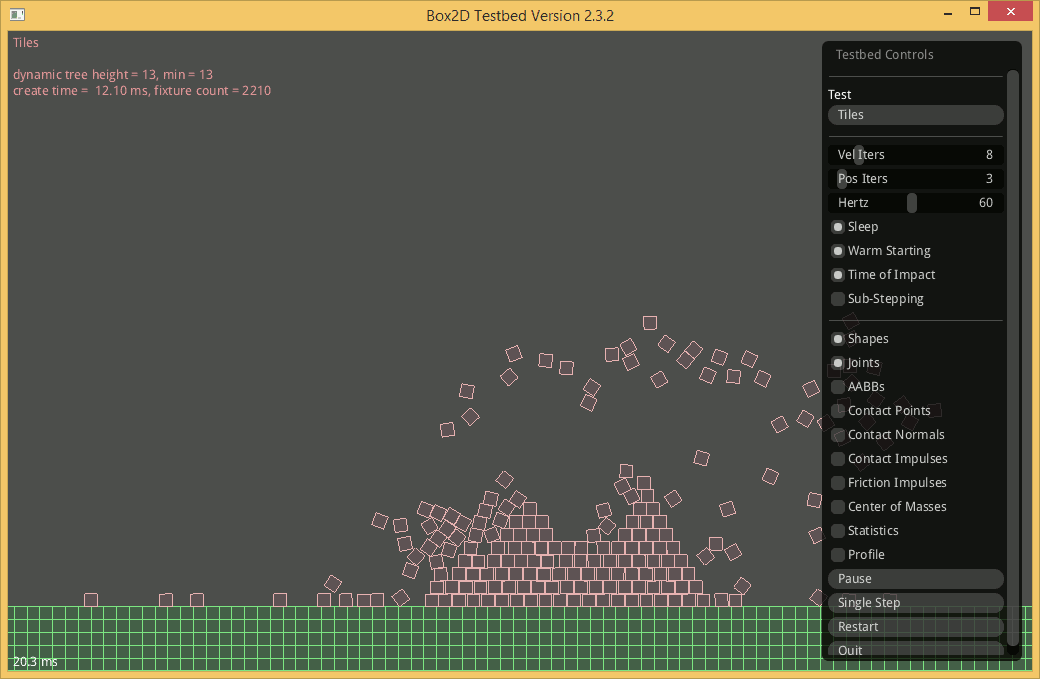
\includegraphics[width=0.9\columnwidth]{windows-05}
    \end{column}

    \begin{column}{6cm}
      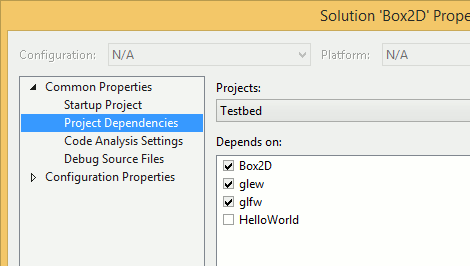
\includegraphics[width=0.9\columnwidth]{windows-06}
    \end{column}
  \end{columns}
\end{frame}

%%%%%%%%%%%%%%%%%%%%%%%%%%%%%%%%%%%%%%%%%%%%%%%%%%%%%%%%%%%%%%%%%%%%%%%%%%%%%%%

\begin{frame}[fragile=singleslide]
  \frametitle{What did you just build?}

  \begin{itemize}
    \item Box2D $\rightarrow$ \emph{Properties}
  \end{itemize}

  \begin{figure}
    \centering
    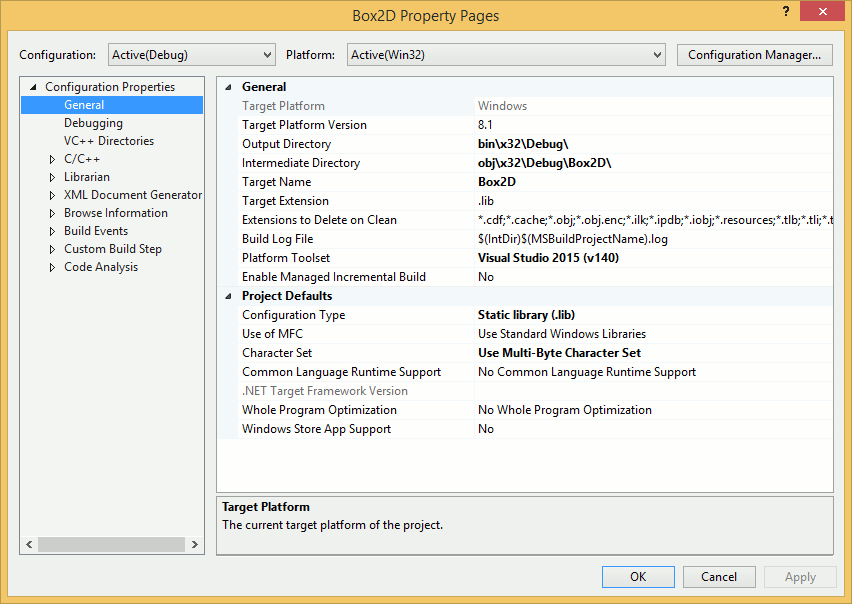
\includegraphics[width=0.8\columnwidth]{windows-07}
  \end{figure}
\end{frame}

%%%%%%%%%%%%%%%%%%%%%%%%%%%%%%%%%%%%%%%%%%%%%%%%%%%%%%%%%%%%%%%%%%%%%%%%%%%%%%%

\begin{frame}[fragile=singleslide]
  \frametitle{Release Builds}

  \begin{itemize}
    \item Run Testbed $\rightarrow$ Enable \emph{Profile}
    \item Note \textcolor{magenta}{\emph{step [ave] (max)}} values
    \item \textcolor{magenta}{\emph{previous [average] (longest time)}} for one physics step in milliseconds
    \item Do it again in Release mode\tikzmark{release}
  \end{itemize}

  \begin{columns}[t]
    \begin{column}{6cm}
      \filename{Debug}
      \begin{figure}
        \centering
        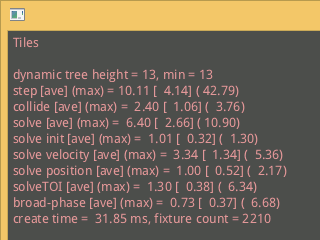
\includegraphics[width=\columnwidth]{windows-08}
      \end{figure}
    \end{column}

    \begin{column}{6cm}
      \filename{Release} 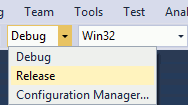
\includegraphics[width=2cm]{windows-release}
      \begin{figure}
        \centering
        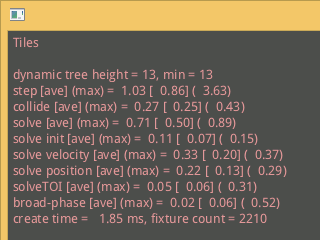
\includegraphics[width=\columnwidth]{windows-09}
      \end{figure}
    \end{column}
  \end{columns}

  
\begin{tikzpicture}[callout]
    \draw \refer{release} -> +(2.5, -1.1);
    \draw (0.41\paperwidth, 0.48\paperheight) node [anchor=south] {\large \textbf{WOW!}} -> (3.5,3) rectangle +(-2em, -1em);
    \draw (0.41\paperwidth, 0.48\paperheight) -> (9.125,3.0625) rectangle +(2em, -1em);
  \end{tikzpicture}

\end{frame}

%%%%%%%%%%%%%%%%%%%%%%%%%%%%%%%%%%%%%%%%%%%%%%%%%%%%%%%%%%%%%%%%%%%%%%%%%%%%%%%

\begin{frame}[fragile=singleslide]
  \frametitle{Creating a Solution}

  \begin{itemize}
    \item Your solution will have multiple projects (your game + libraries)
    \item \emph{File} $\rightarrow$ \emph{New} $\rightarrow$ \emph{Project}
  \end{itemize}

  \begin{figure}
    \centering
    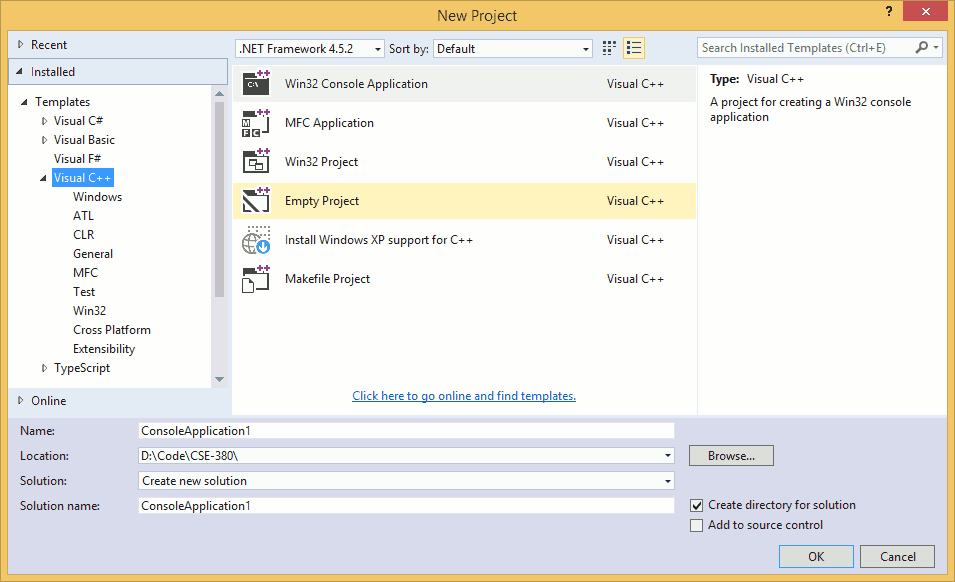
\includegraphics[width=0.85\columnwidth]{windows-10}
  \end{figure}
\end{frame}

%%%%%%%%%%%%%%%%%%%%%%%%%%%%%%%%%%%%%%%%%%%%%%%%%%%%%%%%%%%%%%%%%%%%%%%%%%%%%%%

\begin{frame}[fragile=singleslide]
  \frametitle{Let's Compile Something}

  \begin{itemize}
    \item \emph{Source Files} $\rightarrow$ \emph{Add New Item} $\rightarrow$ \emph{C++ File}
  \end{itemize}

  \cppfile[fontsize=\large]{src/hello.cpp}

\end{frame}

%%%%%%%%%%%%%%%%%%%%%%%%%%%%%%%%%%%%%%%%%%%%%%%%%%%%%%%%%%%%%%%%%%%%%%%%%%%%%%%

\begin{frame}[fragile=singleslide]
  \frametitle{Headers and Classes}

  \begin{itemize}
    \item \emph{Project} $\rightarrow$ \emph{Add} $\rightarrow$ \emph{Class}
    \item \emph{Declare} classes, global functions, etc. in header files (\texttt{.hpp} extension)
    \item \emph{Define} them in a corresponding source file (\texttt{.cpp} extension)
    \begin{itemize}
      \item \textbf{Exception:} \cppinline{template}s must be defined in headers
    \end{itemize}
    \item Reduces the number of files to build
    \begin{itemize}
      \item Header changes? \emph{All \texttt{.cpp} files that use it must be recompiled}
      \item Source changes? Only that file must be recompiled
      \item Prevent linker errors, too
    \end{itemize}
  \end{itemize}
\end{frame}

%%%%%%%%%%%%%%%%%%%%%%%%%%%%%%%%%%%%%%%%%%%%%%%%%%%%%%%%%%%%%%%%%%%%%%%%%%%%%%%

\begin{frame}[fragile=singleslide]
  \frametitle{You Should See These}

  \begin{columns}[t]
    \begin{column}{6cm}
      \filename{Vector2.hpp}
      \cppfile[fontsize=\Large]{src/vector2_1.hpp}
    \end{column}

    \begin{column}{6cm}
      \filename{Vector2.cpp}
      \cppfile[fontsize=\Large]{src/vector2_1.cpp}
    \end{column}
  \end{columns}
\end{frame}

%%%%%%%%%%%%%%%%%%%%%%%%%%%%%%%%%%%%%%%%%%%%%%%%%%%%%%%%%%%%%%%%%%%%%%%%%%%%%%%

\begin{frame}[fragile=singleslide]
  \frametitle{Fleshing It Out}
  
  \begin{columns}[t]
    \begin{column}{5.5cm}
      \filename{Vector2.hpp}
      \cppfile{src/vector2_2.hpp}
    \end{column}

    \begin{column}{6cm}
      \filename{Vector2.cpp}
      \cppfile{src/vector2_2.cpp}
    \end{column}
  \end{columns}
\end{frame}

%%%%%%%%%%%%%%%%%%%%%%%%%%%%%%%%%%%%%%%%%%%%%%%%%%%%%%%%%%%%%%%%%%%%%%%%%%%%%%%

\begin{frame}[fragile=singleslide]
  \frametitle{Do it again, but in 3D}
  
  \begin{columns}[t]
    \begin{column}{5.5cm}
      \filename{Vector3.hpp}
      \cppfile{src/vector3_1.hpp}
    \end{column}

    \begin{column}{6cm}
      \filename{Vector3.cpp}
      \cppfile{src/vector3_1.cpp}
    \end{column}
  \end{columns}
\end{frame}

%%%%%%%%%%%%%%%%%%%%%%%%%%%%%%%%%%%%%%%%%%%%%%%%%%%%%%%%%%%%%%%%%%%%%%%%%%%%%%%

\begin{frame}[fragile=singleslide]
  \frametitle{Add a conversion operator}
  
  \begin{columns}[t]
    \begin{column}{6cm}
      \filename{Vector2.hpp}
      \cppfile[fontsize=\scriptsize]{src/vector2_3.hpp}
    \end{column}

    \begin{column}{6cm}
      \filename{Vector2.cpp}
      \cppfile[fontsize=\scriptsize]{src/vector2_3.cpp}
    \end{column}
  \end{columns}
  
  \begin{itemize}
    \item You just tried a circular \cppinline{#include}!
    \item Won't compile; \texttt{\textbf{incomplete type}}
  \end{itemize}
\end{frame}

%%%%%%%%%%%%%%%%%%%%%%%%%%%%%%%%%%%%%%%%%%%%%%%%%%%%%%%%%%%%%%%%%%%%%%%%%%%%%%%

\begin{frame}[fragile=singleslide]
  \frametitle{What to Do}
  
  \begin{columns}[t]
    \begin{column}{6cm}
      \filename{Vector2.hpp}
      \cppfile[fontsize=\tiny]{src/vector2_4.hpp}
      
      \filename{Vector2.cpp}
      \cppfile[fontsize=\tiny]{src/vector2_4.cpp}
    \end{column}

    \begin{column}{6cm}
      \filename{Vector3.hpp}
      \cppfile[fontsize=\tiny]{src/vector3_2.hpp}
      
      \filename{Vector3.cpp}
      \cppfile[fontsize=\tiny]{src/vector3_2.cpp}
    \end{column}
  \end{columns}
  
  \begin{itemize}
    \item Forward-declare a class when you only need its name
    \begin{itemize}
      \item This is why we split classes into \texttt{.hpp}/\texttt{.cpp}
    \end{itemize}
    \item \cppinline{#include} its header when you need to know what's inside
    \begin{itemize}
      \item i.e. in dependent \texttt{.cpp} files or templates in headers
    \end{itemize}
  \end{itemize}
\end{frame}

%%%%%%%%%%%%%%%%%%%%%%%%%%%%%%%%%%%%%%%%%%%%%%%%%%%%%%%%%%%%%%%%%%%%%%%%%%%%%%%

\begin{frame}[fragile=singleslide]
  \frametitle{Visualized}

  \begin{figure}
    \centering
    \resizebox{0.9\columnwidth}{!}{\input{img/visualized}}
  \end{figure}
\end{frame}

%%%%%%%%%%%%%%%%%%%%%%%%%%%%%%%%%%%%%%%%%%%%%%%%%%%%%%%%%%%%%%%%%%%%%%%%%%%%%%%

\begin{frame}[fragile=singleslide]
  \frametitle{The Problem With Headers}

  \begin{itemize}
    \item Include \cppinline{#pragma once} at the top of each \emph{header}
    \item Otherwise, the contents are defined multiple times
  \end{itemize}

  \begin{figure}
    \begin{tikzpicture}[remember picture]
      \node at (-0.5\paperwidth, 0) [codebox, anchor=west] (include) {\cppinline[fontsize=\tiny]{#include "Texture.hpp"}};
      \node at (-0.05\paperwidth, 0) [anchor=center] (first) {First time included?};
      \node at (0.2\paperwidth, 0.3\paperheight) [codebox, anchor=west] (pragma) {\cppinline[fontsize=\tiny]{// Texture.hpp contents}};
      \node at (0.2\paperwidth, -0.3\paperheight) [codebox, gray, anchor=west] (nothing) {\texttt{\tiny <nothing>}};

      \draw[callout, green] (first.north east) -> (pragma.south west) node [pos=.5, above, sloped, anchor=south] {Yes};
      \draw[callout] (first.south east) -> (nothing.north west) node [pos=.5, above, sloped, anchor=south] {No};
      \draw[callout, black] (include.east) -> (first.west) node [pos=.5, above, sloped, anchor=south] {\cppinline[fontsize=\tiny]{#pragma once}};
    \end{tikzpicture}
  \end{figure}
\end{frame}

%%%%%%%%%%%%%%%%%%%%%%%%%%%%%%%%%%%%%%%%%%%%%%%%%%%%%%%%%%%%%%%%%%%%%%%%%%%%%%%

\begin{frame}[fragile=singleslide]
  \frametitle{The Problem With Headers (cont'd)}

  \begin{columns}[t]
    \begin{column}{6cm}
      \begin{mdframed}[backgroundcolor=red!40]
        \cppfile{src/pragma_france_1.hpp}
      \end{mdframed}
      \begin{mdframed}[backgroundcolor=red!40]
        \cppfile{src/pragma_spain_1.hpp}
      \end{mdframed}
    \end{column}

    \begin{column}{6cm}
      \begin{mdframed}[backgroundcolor=green!40]
        \cppfile{src/pragma_france_2.hpp}
      \end{mdframed}
      \begin{mdframed}[backgroundcolor=green!40]
        \cppfile{src/pragma_spain_2.hpp}
      \end{mdframed}
    \end{column}
  \end{columns}

  \begin{columns}[t]
    \begin{column}{6cm}
      \begin{mdframed}
        \cppfile{src/pragma_main_1.cpp}
      \end{mdframed}
    \end{column}
  \end{columns}

  \begin{columns}[b]
    \begin{column}{6cm}
      \begin{mdframed}[backgroundcolor=red!40]
        \cppfile{src/pragma_main_2.cpp}
      \end{mdframed}
    \end{column}

    \begin{column}{6cm}
      \begin{mdframed}[backgroundcolor=green!40]
        \cppfile{src/pragma_main_3.cpp}
      \end{mdframed}
    \end{column}
  \end{columns}

  \begin{figure}
    \begin{tikzpicture}[remember picture]
    \end{tikzpicture}
  \end{figure}
\end{frame}

%%%%%%%%%%%%%%%%%%%%%%%%%%%%%%%%%%%%%%%%%%%%%%%%%%%%%%%%%%%%%%%%%%%%%%%%%%%%%%%

\begin{frame}[fragile=singleslide]
  \frametitle{Library/Header Install Conventions}

  \begin{columns}[t]
    \begin{column}{4cm}
      \textbf{Package Managers}
      \begin{itemize}
        \item Best bet
        \item Updates automatic
        \item \href{https://www.nuget.org/}{NuGet} on Windows
        \item \href{http://brew.sh/}{Homebrew} on Mac
        \item Included on Linux (usually \texttt{apt-get})
      \end{itemize}
    \end{column}

    \begin{column}{4cm}
      \textbf{Manual Install}
      \begin{itemize}
        \item Next best thing
        \item Hopefully there's a build system
        \item Otherwise, God help you
      \end{itemize}
    \end{column}

    \begin{column}{4cm}
      \textbf{In-Project}
      \begin{itemize}
        \item Avoid in real life
        \item Updates must be manual
        \item Source repo is larger
        \item Last resort
        \begin{itemize}
          \item Box2D doesn't have a NuGet package
          \item \href{http://www.grinninglizard.com/tinyxml2/}{tinyxml} does
        \end{itemize}
      \end{itemize}
    \end{column}
  \end{columns}
\end{frame}

%%%%%%%%%%%%%%%%%%%%%%%%%%%%%%%%%%%%%%%%%%%%%%%%%%%%%%%%%%%%%%%%%%%%%%%%%%%%%%%

\begin{frame}[fragile=singleslide]
  \frametitle{Importing Box2D}
  \begin{figure}
    \centering
    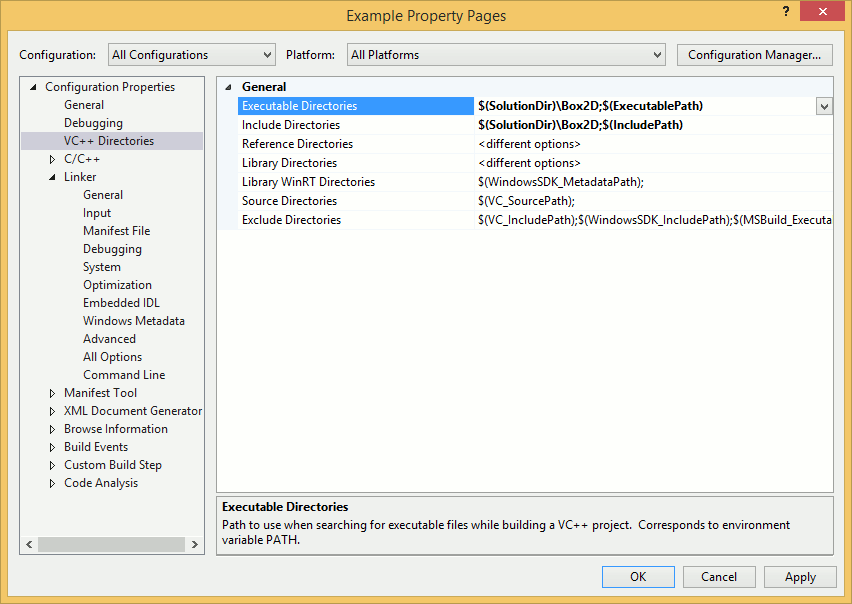
\includegraphics[width=0.9\columnwidth]{windows-dir}
  \end{figure}
\end{frame}

%%%%%%%%%%%%%%%%%%%%%%%%%%%%%%%%%%%%%%%%%%%%%%%%%%%%%%%%%%%%%%%%%%%%%%%%%%%%%%%

\begin{frame}[fragile=singleslide]
  \frametitle{Configuration Macros}
  \begin{figure}
    \centering
    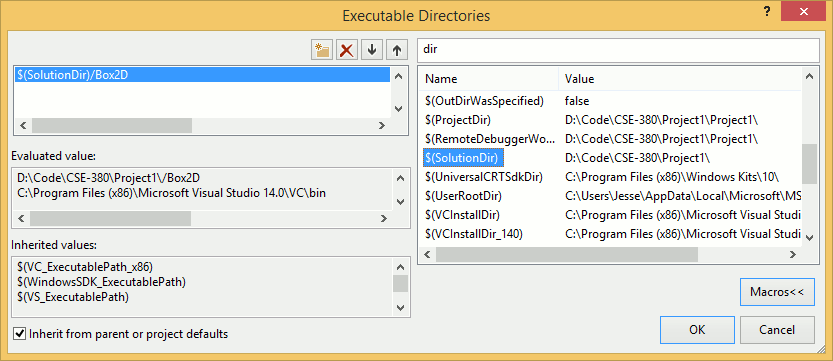
\includegraphics[width=0.9\columnwidth]{windows-macro}
  \end{figure}
\end{frame}

%%%%%%%%%%%%%%%%%%%%%%%%%%%%%%%%%%%%%%%%%%%%%%%%%%%%%%%%%%%%%%%%%%%%%%%%%%%%%%%

\begin{frame}[fragile=singleslide]
  \frametitle{Almost There...}
  
  \filename{main.cpp}
  \cppfile[fontsize=\scriptsize]{src/main.cpp}
\end{frame}

%%%%%%%%%%%%%%%%%%%%%%%%%%%%%%%%%%%%%%%%%%%%%%%%%%%%%%%%%%%%%%%%%%%%%%%%%%%%%%%

\begin{frame}[fragile=singleslide]
  \frametitle{Oh, No, Wait}

  \begin{figure}
    \centering
    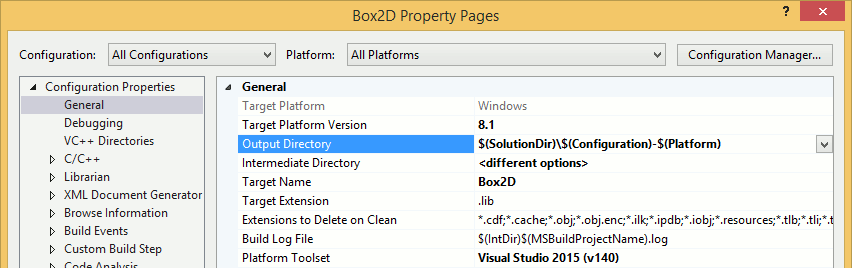
\includegraphics[width=\columnwidth]{windows-11}
  \end{figure}

  \begin{figure}
    \centering
    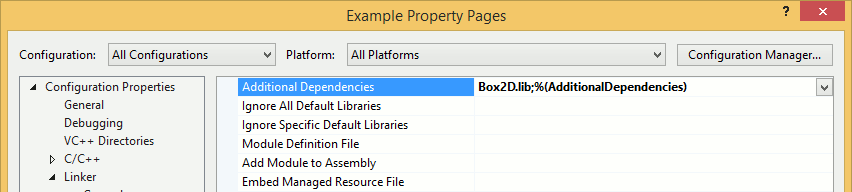
\includegraphics[width=\columnwidth]{windows-12}
  \end{figure}
\end{frame}

%%%%%%%%%%%%%%%%%%%%%%%%%%%%%%%%%%%%%%%%%%%%%%%%%%%%%%%%%%%%%%%%%%%%%%%%%%%%%%%

\begin{frame}[fragile=singleslide]
  \frametitle{Success!}

  \begin{figure}
    \centering
    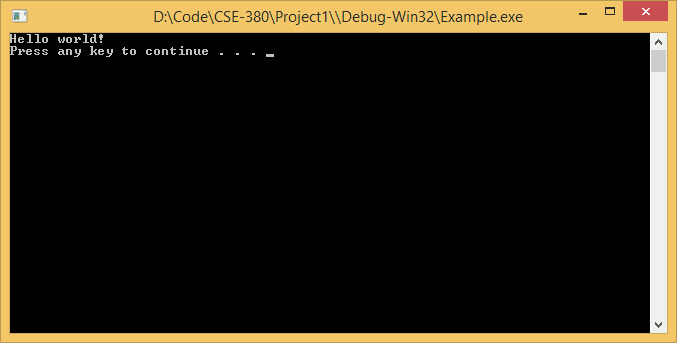
\includegraphics[width=\columnwidth]{windows-hello}
  \end{figure}
\end{frame}

%%%%%%%%%%%%%%%%%%%%%%%%%%%%%%%%%%%%%%%%%%%%%%%%%%%%%%%%%%%%%%%%%%%%%%%%%%%%%%%

\begin{frame}[fragile=singleslide]
  \frametitle{Using the Debugger}

  \begin{figure}
    \centering
    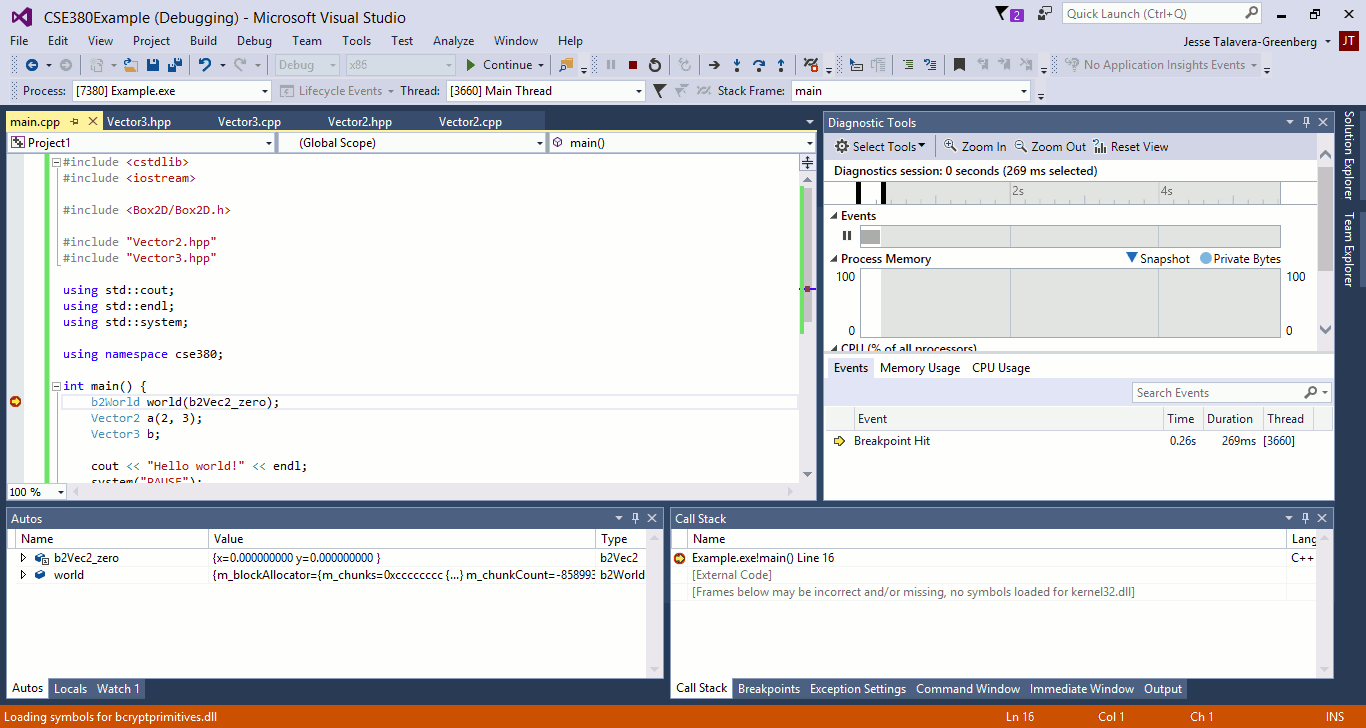
\includegraphics[width=\columnwidth]{windows-debug}

    \begin{tikzpicture}[callout]
      \draw (-3, 4) node (debug_remember) [anchor=west] {Pretty much the same, but\\remember to use Debug builds} -> (-5.8, 3.375);
      \draw (debug_remember.south west) -> (-5.5, 2);
      \draw (debug_remember.north) -> (.5, 6.25);
      \draw (debug_remember.south) -> (0, 2.5);
    \end{tikzpicture}
  \end{figure}

\end{frame}

%%%%%%%%%%%%%%%%%%%%%%%%%%%%%%%%%%%%%%%%%%%%%%%%%%%%%%%%%%%%%%%%%%%%%%%%%%%%%%%

\begin{frame}[fragile=singleslide]
  \frametitle{\href{http://doxygen.org/}{Doxygen}}

  \begin{itemize}
    \item De facto standard C++ documentation tool
    \item Similar tags and syntax to Javadoc
    \item More powerful
  \end{itemize}

  \cppfile[fontsize=\scriptsize]{src/doxygen.cpp}
\end{frame}

%%%%%%%%%%%%%%%%%%%%%%%%%%%%%%%%%%%%%%%%%%%%%%%%%%%%%%%%%%%%%%%%%%%%%%%%%%%%%%%

\begin{frame}[fragile=singleslide]
  \frametitle{\href{https://cmake.org/}{CMake}}

  \begin{columns}[t]
    \begin{column}{5cm}
      \begin{itemize}
        \item Meta-build system
        \begin{itemize}
          \item Makefiles, Visual Studio projects, etc.
        \end{itemize}
        \item Popular choice for cross-platform C++ projects
      \end{itemize}
    \end{column}

    \begin{column}{7cm}
      \cmakefile{src/cmake.cmake}
    \end{column}
  \end{columns}
\end{frame}

%%%%%%%%%%%%%%%%%%%%%%%%%%%%%%%%%%%%%%%%%%%%%%%%%%%%%%%%%%%%%%%%%%%%%%%%%%%%%%%

\begin{frame}[fragile=singleslide]
  \frametitle{Popular C++ Libraries}

  \begin{columns}[t]
    \begin{column}{4cm}
      \textbf{\href{http://www.boost.org/}{Boost}}
      \begin{itemize}
        \item Huge utility library
        \begin{itemize}
          \item Image processing
          \item Geometry
          \item File systems
          \item Graph theory
          \item Networking
          \item Unit testing
          \item Lots, lots more
        \end{itemize}
        \item Considered essential
        \item No, seriously, it's a real motherfucker
      \end{itemize}
    \end{column}

    \begin{column}{4cm}
      \textbf{\href{http://www.qt.io/}{Qt}}
      \begin{itemize}
        \item Big-ass framework
        \item Provides its own tools
        \begin{itemize}
          \item GUI builder
          \item Custom build system
          \item Asset management (images, etc.)
        \end{itemize}
        \item Cross-platform
        \item Not well-suited for games

      \end{itemize}
    \end{column}

    \begin{column}{4cm}
      \textbf{\href{http://www.sfml-dev.org/}{SFML}}
      \begin{itemize}
        \item Multimedia framework
        \begin{itemize}
          \item Graphics
          \item Sound
          \item Input handling
          \item Networking
        \end{itemize}
        \item Simple to use, good for beginners (you)
        \item Cross-platform (uses OpenGL)
        \item Follows good C++ practices without being complicated
      \end{itemize}
    \end{column}
  \end{columns}
\end{frame}

%%%%%%%%%%%%%%%%%%%%%%%%%%%%%%%%%%%%%%%%%%%%%%%%%%%%%%%%%%%%%%%%%%%%%%%%%%%%%%%

\begin{frame}[fragile=singleslide]
  \frametitle{Next Week}

  \begin{itemize}
    \item \href{http://git-scm.com/}{Something completely different}
  \end{itemize}

  \begin{figure}
    \centering
    
\includegraphics[width=0.65\columnwidth]{octocat}
  \end{figure}
\end{frame}

\end{document}